\documentclass[]{article}
\usepackage{lmodern}
\usepackage{amssymb,amsmath}
\usepackage{ifxetex,ifluatex}
\usepackage{fixltx2e} % provides \textsubscript
\ifnum 0\ifxetex 1\fi\ifluatex 1\fi=0 % if pdftex
  \usepackage[T1]{fontenc}
  \usepackage[utf8]{inputenc}
\else % if luatex or xelatex
  \ifxetex
    \usepackage{mathspec}
  \else
    \usepackage{fontspec}
  \fi
  \defaultfontfeatures{Ligatures=TeX,Scale=MatchLowercase}
  \newcommand{\euro}{€}
    \setmainfont[]{Arial}
\fi
% use upquote if available, for straight quotes in verbatim environments
\IfFileExists{upquote.sty}{\usepackage{upquote}}{}
% use microtype if available
\IfFileExists{microtype.sty}{%
\usepackage{microtype}
\UseMicrotypeSet[protrusion]{basicmath} % disable protrusion for tt fonts
}{}


\usepackage{longtable,booktabs}
\usepackage{graphicx,grffile}
\makeatletter
\def\maxwidth{\ifdim\Gin@nat@width>\linewidth\linewidth\else\Gin@nat@width\fi}
\def\maxheight{\ifdim\Gin@nat@height>\textheight\textheight\else\Gin@nat@height\fi}
\makeatother
% Scale images if necessary, so that they will not overflow the page
% margins by default, and it is still possible to overwrite the defaults
% using explicit options in \includegraphics[width, height, ...]{}
\setkeys{Gin}{width=\maxwidth,height=\maxheight,keepaspectratio}
\setlength{\parindent}{0pt}
\setlength{\parskip}{6pt plus 2pt minus 1pt}
\setlength{\emergencystretch}{3em}  % prevent overfull lines
\providecommand{\tightlist}{%
  \setlength{\itemsep}{0pt}\setlength{\parskip}{0pt}}
\setcounter{secnumdepth}{5}

%%% Use protect on footnotes to avoid problems with footnotes in titles
\let\rmarkdownfootnote\footnote%
\def\footnote{\protect\rmarkdownfootnote}

%%% Change title format to be more compact
\usepackage{titling}

\RequirePackage[]{/mnt/isilon/cbmi/tan_lab/pengt/R/library/BiocStyle/resources/tex/Bioconductor2}

% Create subtitle command for use in maketitle
\newcommand{\subtitle}[1]{
  \posttitle{
    \begin{center}\large#1\end{center}
    }
}

\setlength{\droptitle}{-2em}
\bioctitle[]{Introduction to SCRABBLE}
  \pretitle{\vspace{\droptitle}\centering\huge}
  \posttitle{\par}
\author{Tao Peng}
  \preauthor{\centering\large\emph}
  \postauthor{\par}
  \predate{\centering\large\emph}
  \postdate{\par}
  \date{Updated on 2018-06-15}


% Redefines (sub)paragraphs to behave more like sections
\ifx\paragraph\undefined\else
\let\oldparagraph\paragraph
\renewcommand{\paragraph}[1]{\oldparagraph{#1}\mbox{}}
\fi
\ifx\subparagraph\undefined\else
\let\oldsubparagraph\subparagraph
\renewcommand{\subparagraph}[1]{\oldsubparagraph{#1}\mbox{}}
\fi

% code highlighting
\definecolor{fgcolor}{rgb}{0.251, 0.251, 0.251}
\newcommand{\hlnum}[1]{\textcolor[rgb]{0.816,0.125,0.439}{#1}}%
\newcommand{\hlstr}[1]{\textcolor[rgb]{0.251,0.627,0.251}{#1}}%
\newcommand{\hlcom}[1]{\textcolor[rgb]{0.502,0.502,0.502}{\textit{#1}}}%
\newcommand{\hlopt}[1]{\textcolor[rgb]{0,0,0}{#1}}%
\newcommand{\hlstd}[1]{\textcolor[rgb]{0.251,0.251,0.251}{#1}}%
\newcommand{\hlkwa}[1]{\textcolor[rgb]{0.125,0.125,0.941}{#1}}%
\newcommand{\hlkwb}[1]{\textcolor[rgb]{0,0,0}{#1}}%
\newcommand{\hlkwc}[1]{\textcolor[rgb]{0.251,0.251,0.251}{#1}}%
\newcommand{\hlkwd}[1]{\textcolor[rgb]{0.878,0.439,0.125}{#1}}%
\let\hlipl\hlkwb
%
\usepackage{fancyvrb}
\newcommand{\VerbBar}{|}
\newcommand{\VERB}{\Verb[commandchars=\\\{\}]}
\DefineVerbatimEnvironment{Highlighting}{Verbatim}{commandchars=\\\{\}}
%
\newenvironment{Shaded}{\begin{myshaded}}{\end{myshaded}}
% set background for result chunks
\let\oldverbatim\verbatim
\renewenvironment{verbatim}{\color{codecolor}\begin{myshaded}\begin{oldverbatim}}{\end{oldverbatim}\end{myshaded}}
%
\newcommand{\KeywordTok}[1]{\hlkwd{#1}}
\newcommand{\DataTypeTok}[1]{\hlkwc{#1}}
\newcommand{\DecValTok}[1]{\hlnum{#1}}
\newcommand{\BaseNTok}[1]{\hlnum{#1}}
\newcommand{\FloatTok}[1]{\hlnum{#1}}
\newcommand{\ConstantTok}[1]{\hlnum{#1}}
\newcommand{\CharTok}[1]{\hlstr{#1}}
\newcommand{\SpecialCharTok}[1]{\hlstr{#1}}
\newcommand{\StringTok}[1]{\hlstr{#1}}
\newcommand{\VerbatimStringTok}[1]{\hlstr{#1}}
\newcommand{\SpecialStringTok}[1]{\hlstr{#1}}
\newcommand{\ImportTok}[1]{{#1}}
\newcommand{\CommentTok}[1]{\hlcom{#1}}
\newcommand{\DocumentationTok}[1]{\hlcom{#1}}
\newcommand{\AnnotationTok}[1]{\hlcom{#1}}
\newcommand{\CommentVarTok}[1]{\hlcom{#1}}
\newcommand{\OtherTok}[1]{{#1}}
\newcommand{\FunctionTok}[1]{\hlstd{#1}}
\newcommand{\VariableTok}[1]{\hlstd{#1}}
\newcommand{\ControlFlowTok}[1]{\hlkwd{#1}}
\newcommand{\OperatorTok}[1]{\hlopt{#1}}
\newcommand{\BuiltInTok}[1]{{#1}}
\newcommand{\ExtensionTok}[1]{{#1}}
\newcommand{\PreprocessorTok}[1]{\textit{#1}}
\newcommand{\AttributeTok}[1]{{#1}}
\newcommand{\RegionMarkerTok}[1]{{#1}}
\newcommand{\InformationTok}[1]{\textcolor{messagecolor}{#1}}
\newcommand{\WarningTok}[1]{\textcolor{warningcolor}{#1}}
\newcommand{\AlertTok}[1]{\textcolor{errorcolor}{#1}}
\newcommand{\ErrorTok}[1]{\textcolor{errorcolor}{#1}}
\newcommand{\NormalTok}[1]{\hlstd{#1}}
%
\AtBeginDocument{\bibliographystyle{/mnt/isilon/cbmi/tan_lab/pengt/R/library/BiocStyle/resources/tex/unsrturl}}

\begin{document}
\maketitle

\packageVersion{SCRABBLE 0.2.0}

{
\setcounter{tocdepth}{2}
\tableofcontents
\newpage
}
\begin{Shaded}
\begin{Highlighting}[]
 \KeywordTok{library}\NormalTok{(SCRABBLE)}
\end{Highlighting}
\end{Shaded}

\section{Simulation Data Study}\label{simulation-data-study}

\subsection{Data Generation}\label{data-generation}

The data set was generated from down sampling from bulk RNAseq data. We
used the bulk RNA-Seq data set of mouse hair follicles (GSE85039). In
total, the dataset contains 20 different combinations of anatomic sites
and developmental time points, thus constituting a high dimensional
measurement space. We used the following procedures to generate the
drop-out datasets. 1) We selected 732 genes that are differentially
expressed in the 20 conditions based on ANOVA analysis. 2) We randomly
selected 10 out of the 20 conditions. 3) For each condition, we
generated 100 resampled datasets. The means and standard deviations of
genes were calculated for each condition based on the 100 resampled
datasets. 4) 100 new datasets were generated based on the mean and the
standard deviation of each gene. 5) The final data set was obtained by
combining 1000 samples representing the 10 conditions. This 1000x732
matrix now represents 1000 cells and 732 genes. 6) we make the drop-out
rate of each gene in each cell following a double exponential function .
Zero values are introduced into the simulated data for each gene in each
cell based on the Bernoulli distribution defined by the corresponding
drop-out rate.

\subsubsection{Load the data}\label{load-the-data}

\begin{Shaded}
\begin{Highlighting}[]
\NormalTok{data_sc <-}\StringTok{ }\NormalTok{data[[}\DecValTok{1}\NormalTok{]]}
\NormalTok{data_bulk <-}\StringTok{ }\NormalTok{data[[}\DecValTok{2}\NormalTok{]]}
\NormalTok{data_true <-}\StringTok{ }\NormalTok{data[[}\DecValTok{3}\NormalTok{]]}
\end{Highlighting}
\end{Shaded}

\subsubsection{Plot the data}\label{plot-the-data}

\begin{Shaded}
\begin{Highlighting}[]
\NormalTok{pl <-}\StringTok{ }\KeywordTok{list}\NormalTok{()}
\NormalTok{pl[[}\DecValTok{1}\NormalTok{]] <-}\StringTok{ }\KeywordTok{plot_data}\NormalTok{(}\KeywordTok{log10}\NormalTok{(data_true }\OperatorTok{+}\StringTok{ }\DecValTok{1}\NormalTok{),}\StringTok{"True Data"}\NormalTok{)}
\NormalTok{pl[[}\DecValTok{2}\NormalTok{]] <-}\StringTok{ }\KeywordTok{plot_data}\NormalTok{(}\KeywordTok{log10}\NormalTok{(data_sc }\OperatorTok{+}\StringTok{ }\DecValTok{1}\NormalTok{),}\StringTok{"Drop-out Data"}\NormalTok{)}
\NormalTok{main <-}\StringTok{ }\NormalTok{gridExtra}\OperatorTok{::}\KeywordTok{grid.arrange}\NormalTok{(}\DataTypeTok{grobs =}\NormalTok{ pl,}\DataTypeTok{ncol =} \DecValTok{2}\NormalTok{, }\DataTypeTok{top =} \StringTok{""}\NormalTok{)}
\end{Highlighting}
\end{Shaded}

\begin{adjustwidth}{\fltoffset}{0mm}
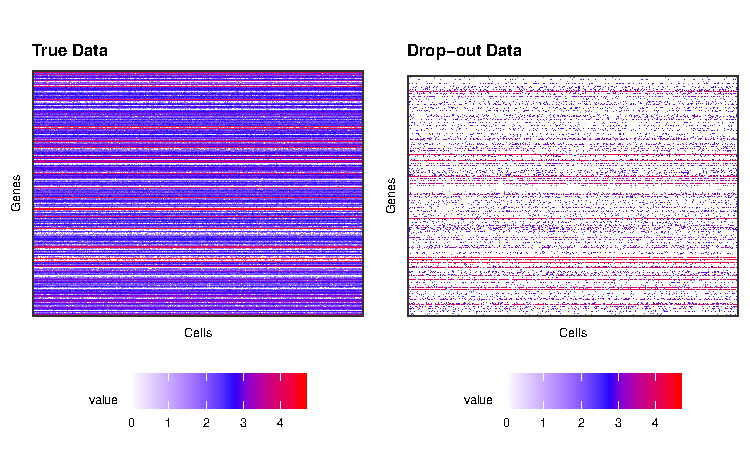
\includegraphics{my-vignette_files/figure-latex/unnamed-chunk-3-1} \end{adjustwidth}

\subsection{Run SCRABBLE}\label{run-scrabble}

SCRABBLE imputes drop-out data by optimizing an objective function that
consists of three terms. The first term ensures that imputed values for
genes with nonzero expression remain as close to their original values
as possible, thus minimizing unwanted bias towards expressed genes. The
second term ensures the rank of the imputed data matrix to be as small
as possible. The rationale is that we only expect a limited number of
distinct cell types in the samples. The third term operates on the bulk
RNA-Seq data. It ensures consistency between the average gene expression
of the aggregated imputed data and the average gene expression of the
bulk RNA-Seq data. We developed 58 a convex optimization algorithm to
minimize the objective function.

\subsubsection{Set up the parameter used in
SCRABBLE}\label{set-up-the-parameter-used-in-scrabble}

\begin{Shaded}
\begin{Highlighting}[]
\NormalTok{parameter <-}\StringTok{ }\KeywordTok{c}\NormalTok{(}\DecValTok{100}\NormalTok{,}\FloatTok{2e-7}\NormalTok{)}
\NormalTok{nIter <-}\StringTok{ }\DecValTok{100}
\end{Highlighting}
\end{Shaded}

\subsubsection{Run SCRABLE}\label{run-scrable}

\begin{Shaded}
\begin{Highlighting}[]
\NormalTok{result <-}\StringTok{ }\KeywordTok{scrabble}\NormalTok{(data, }\DataTypeTok{parameter =}\NormalTok{ parameter, }\DataTypeTok{nIter =}\NormalTok{ nIter, }\DataTypeTok{error_out_threshold =} \FloatTok{1e-05}\NormalTok{, }\DataTypeTok{nIter_inner =} \DecValTok{5}\NormalTok{, }\DataTypeTok{error_inner_threshold =} \FloatTok{1e-05}\NormalTok{)}
\CommentTok{#> [1] "SCRABBLE begins the imputation of the data with 732 genes and 1000 cells"}
\CommentTok{#> [1] "Imputation initialization is finished"}
\CommentTok{#> [1] "... ...."}
\CommentTok{#> [1] "Imputation is finished"}
\end{Highlighting}
\end{Shaded}

\subsubsection{Plot the data}\label{plot-the-data-1}

\begin{Shaded}
\begin{Highlighting}[]
\NormalTok{pl <-}\StringTok{ }\KeywordTok{list}\NormalTok{()}
\NormalTok{pl[[}\DecValTok{1}\NormalTok{]] <-}\StringTok{ }\KeywordTok{plot_data}\NormalTok{(}\KeywordTok{log10}\NormalTok{(data[[}\DecValTok{3}\NormalTok{]] }\OperatorTok{+}\StringTok{ }\DecValTok{1}\NormalTok{),}\StringTok{"True Data"}\NormalTok{)}
\NormalTok{pl[[}\DecValTok{2}\NormalTok{]] <-}\StringTok{ }\KeywordTok{plot_data}\NormalTok{(}\KeywordTok{log10}\NormalTok{(data[[}\DecValTok{1}\NormalTok{]] }\OperatorTok{+}\StringTok{ }\DecValTok{1}\NormalTok{),}\StringTok{"Drop-out Data"}\NormalTok{)}
\NormalTok{pl[[}\DecValTok{3}\NormalTok{]] <-}\StringTok{ }\KeywordTok{plot_data}\NormalTok{(}\KeywordTok{log10}\NormalTok{(result }\OperatorTok{+}\StringTok{ }\DecValTok{1}\NormalTok{),}\StringTok{"Imputed by SCRABBLE"}\NormalTok{)}
\NormalTok{main <-}\StringTok{ }\NormalTok{gridExtra}\OperatorTok{::}\KeywordTok{grid.arrange}\NormalTok{(}\DataTypeTok{grobs =}\NormalTok{ pl, }\DataTypeTok{ncol =} \DecValTok{3}\NormalTok{, }\DataTypeTok{top =} \StringTok{""}\NormalTok{)}
\end{Highlighting}
\end{Shaded}

\begin{adjustwidth}{\fltoffset}{0mm}
\includegraphics{my-vignette_files/figure-latex/unnamed-chunk-6-1} \end{adjustwidth}

\section{SessionInfo}\label{sessioninfo}

\begin{Shaded}
\begin{Highlighting}[]
\KeywordTok{sessionInfo}\NormalTok{()}
\CommentTok{#> R version 3.4.4 (2018-03-15)}
\CommentTok{#> Platform: x86_64-redhat-linux-gnu (64-bit)}
\CommentTok{#> Running under: Red Hat Enterprise Linux}
\CommentTok{#> }
\CommentTok{#> Matrix products: default}
\CommentTok{#> BLAS/LAPACK: /usr/lib64/R/lib/libRblas.so}
\CommentTok{#> }
\CommentTok{#> locale:}
\CommentTok{#>  [1] LC_CTYPE=en_US.UTF-8       LC_NUMERIC=C              }
\CommentTok{#>  [3] LC_TIME=en_US.UTF-8        LC_COLLATE=en_US.UTF-8    }
\CommentTok{#>  [5] LC_MONETARY=en_US.UTF-8    LC_MESSAGES=en_US.UTF-8   }
\CommentTok{#>  [7] LC_PAPER=en_US.UTF-8       LC_NAME=C                 }
\CommentTok{#>  [9] LC_ADDRESS=C               LC_TELEPHONE=C            }
\CommentTok{#> [11] LC_MEASUREMENT=en_US.UTF-8 LC_IDENTIFICATION=C       }
\CommentTok{#> }
\CommentTok{#> attached base packages:}
\CommentTok{#> [1] stats     graphics  grDevices utils     datasets  methods   base     }
\CommentTok{#> }
\CommentTok{#> other attached packages:}
\CommentTok{#> [1] SCRABBLE_0.2.0  BiocStyle_2.6.1}
\CommentTok{#> }
\CommentTok{#> loaded via a namespace (and not attached):}
\CommentTok{#>  [1] Rcpp_0.12.16       pracma_2.1.4       RSpectra_0.12-0   }
\CommentTok{#>  [4] pillar_1.2.1       compiler_3.4.4     RColorBrewer_1.1-2}
\CommentTok{#>  [7] plyr_1.8.4         tools_3.4.4        digest_0.6.15     }
\CommentTok{#> [10] memoise_1.1.0      evaluate_0.10.1    tibble_1.4.2      }
\CommentTok{#> [13] gtable_0.2.0       lattice_0.20-35    rlang_0.2.0       }
\CommentTok{#> [16] Matrix_1.2-12      rstudioapi_0.7     commonmark_1.5    }
\CommentTok{#> [19] yaml_2.1.18        xfun_0.1           gridExtra_2.3     }
\CommentTok{#> [22] withr_2.1.1        stringr_1.3.1      knitr_1.20        }
\CommentTok{#> [25] roxygen2_6.0.1     xml2_1.2.0         desc_1.2.0        }
\CommentTok{#> [28] devtools_1.13.5    rprojroot_1.3-2    grid_3.4.4        }
\CommentTok{#> [31] R6_2.2.2           rARPACK_0.11-0     bookdown_0.7      }
\CommentTok{#> [34] rmarkdown_1.9      ggplot2_2.2.1      reshape2_1.4.3    }
\CommentTok{#> [37] magrittr_1.5       scales_0.5.0       backports_1.1.2   }
\CommentTok{#> [40] htmltools_0.3.6    assertthat_0.2.0   colorspace_1.3-2  }
\CommentTok{#> [43] labeling_0.3       stringi_1.2.2      lazyeval_0.2.1    }
\CommentTok{#> [46] munsell_0.4.3      crayon_1.3.4}
\end{Highlighting}
\end{Shaded}

\end{document}
